


  Lines $l$ and $s$ are tangent to the circle (centered at $C$) at points $A$ and $B$.

\begin{center}
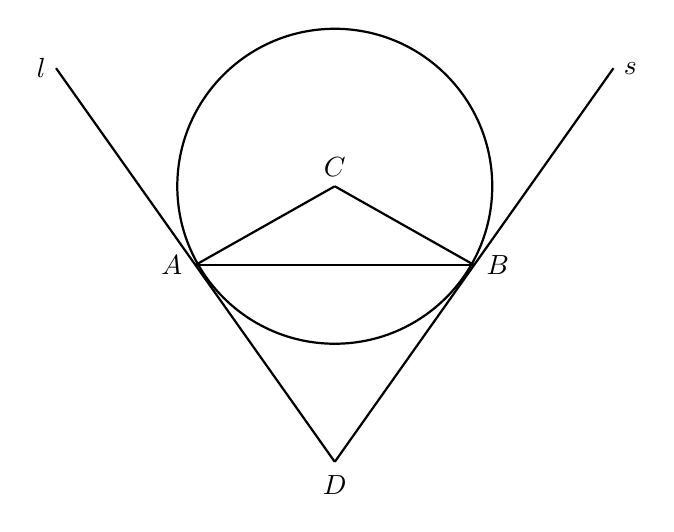
\begin{tikzpicture}
    \draw[thick] (0,0) circle (2cm);
    \draw[thick] (0,-3.5)--(-1.77-1.77,-1+2.5) node[sloped, left]{$l$};              
     \draw[thick] (0,-3.5)--(+1.77+1.77,-1+2.5) node[sloped, right]{$s$};
     
     \draw[thick] (0,0)--(-1.77,-1);
     \node[above] (0,0) {$C$};    
     \draw node at (-1.77-.3,-1) {$A$};
     \draw node at (1.77+.3,-1) {$B$};              
     
          \draw node at (0,-3.8) {$D$};     
     \draw[thick] (0,0)--(1.77,-1); 
       \draw[thick] (-1.77,-1)--(1.77,-1);    
\end{tikzpicture}
\end{center}
Which of the following must be true?

\begin{enumerate}[label=\Roman*.]
\item $m\angle CAB=m\angle ABD$ 
\item $m\angle BAD=m\angle ABD$ 
\item If $m\angle ACB=90^\circ$, then quadrilateral $ACBD$ is a rectangle.
\end{enumerate}




\ifsat
	\begin{enumerate}[label=\Alph*)]
		\item  I only 
		\item  II only
		\item  III only
		\item  II and III only %
	\end{enumerate}
\else
\fi

\ifacteven
	\begin{enumerate}[label=\textbf{\Alph*.},itemsep=\fill,align=left]
		\setcounter{enumii}{5}
		\item  I only 
		\item  II only
		\item  III only
		\addtocounter{enumii}{1}
		\item  II and III only %
		\item  I, II and III
	\end{enumerate}
\else
\fi

\ifactodd
	\begin{enumerate}[label=\textbf{\Alph*.},itemsep=\fill,align=left]
		\item  I only 
		\item  II only
		\item  III only
		\item  II and III only %
		\item  I, II and III
	\end{enumerate}
\else
\fi

\ifgridin
  II and III only %

\else
\fi

